\chapter{Point Cloud Visibility}
\label{ch:visibility}
This chapter introduces our custom point cloud visibility algorithm. It starts by giving in Section~\ref{sc:spec-visibility}, a clear context for the presented work. Then, Section~\ref{sc:related-visibility} gives an overview of the previous related work and describes some experimentations previously-published point cloud visibility algorithms. Finally, as nothing seems to be well adjusted for our specific case we implemented a custom point cloud visibility algorithm described in Section~\ref{sc:custom}.

\section{Specifications}
\label{sc:spec-visibility}

\subsection{Context}
Currently in \CC, there is a way to still use a point cloud for reconstructing purposes even if the scanner's location information is lost. It gives the user the opportunity to manually set the scanners position on a 3D representation of the point cloud. But, only one position can be set. It requires that the point cloud contains points resulting from \emph{one and only one} scanner\footnote{Also known as monoscan point cloud.}. This is because, during the reconstruction, \CC uses
the scanner location to orient the normals at each point. In a monoscan point cloud case, it simply orients each normal toward the scanner. But in case of multiscan point cloud, it needs to know for each point, toward which scanner the normal must be oriented, which is difficult to find.

Therefore, even if \emph{ScanFinder} (Chapter~\ref{ch:scanfinder}) is applied on a LAS format\footnote{A point cloud format that \CC wants to support and which does not store scanner locations in its metadata.} multiscan point cloud in order to retrieve all scanner positions, the reconstruction is still infeasible for \CC. This is where a point cloud visibility algorithm is useful in order to attribute each point to a scanner. Have in mind that a point can be seen by two scanners, especially if there is no physical barrier between them. In this case it is difficult to exactly know which scanner produced the point. But, as this point-scanner attribution is only required for normal orientations, we only need to know which scanner best sees it.

\subsection{Objective}
\label{subsc:vis-objective}
As a final step toward supporting point clouds without scanner locations, the algorithm must:
\begin{itemize}
\item take as input any 3D point cloud captured from static scanners as well as the location of all scanners,
\item be invariant to differences between scanners, such as: density, noise, rotation angle,
\item find for each point the scanner which best sees it, not necessary the scanner which produced it,
\item have a reasonnable running time.
\end{itemize}

As for \emph{ScanFinder} described in Chapter~\ref{ch:scanfinder}, the algorithm is not expected to work with mobile point clouds.


\section{Related work}
\label{sc:related-visibility}
This section highlights some previous work (Section~\ref{subsc:visibility-prev}) on the subject of \emph{Point cloud visibility} and describes two previously-published algorithms and their results.


\subsection{Previous work}
\label{subsc:visibility-prev}
Visibility in point clouds is a topic that experienced several publications since the 1960s~\cite{appel, sutherland, funkhouser, greene, bittner}. Some methods solve this problem in a 3D rendering context by estimating normals and reconstructing surfaces \cite{sainz1, sainz2, wald, wu}. This contrasts with our case as we need visible points in order to reconstruct surfaces. Another common approach is to use z-buffering techniques based on point depths~\cite{dachsbacher} to reconstruct
surfaces in a real-time rendering context. Even if this approach can be adapted to compute visibility of all points from all scanner location viewpoints, it is not robust to noisy point clouds.

One elegant approach computes point cloud visibility without surface reconstruction: \cite{vis1}. This approach is invariant to point cloud density and only point coordinates are needed (no normal estimation). It uses simple operations: an inversion followed by a convex hull computation. However, it is not robust enough against point cloud noises. An improved version \cite{vis2} has been published, it improves handling of noise and concave surfaces in point clouds.
We tried both algorithms. They are described in Section~\ref{subsc:direct} and Section~\ref{subsc:noisy} as well as the obtained results.


\subsection{\emph{Direct Visibility of Point Sets}}
\label{subsc:direct}

\subsubsection{Overview}
The purpose of \cite{vis1} is to detect direclty which points of a point cloud are visible from a specific point of view. The problem being solved can be formalised as such: Given a set of points $P$ (considered a sampling of continuous surface $S$) and a viewpoint $C$, determine the points in $P$ visible from $C$. They introduced the HPR (Hidden Point Removal) Operator. This operator uses two simple operations:

\begin{itemize}
  \item an inversion
  \item a convex hull computation
\end{itemize}

A spherical inversion based on the depth of the points put the nearest points (must of them visible) further away. The second step on the right, based on a convex hull computation, detects visible points. A point lying on this convex hull is considered as visible. Even if a visible point is far in the real domain and closer in the inverted domain it should be on this convex hull, as long as it is visible -- no points behind it, no points hidding it.

\subsubsection{Results and discussions}
\begin{figure}
  \centering
  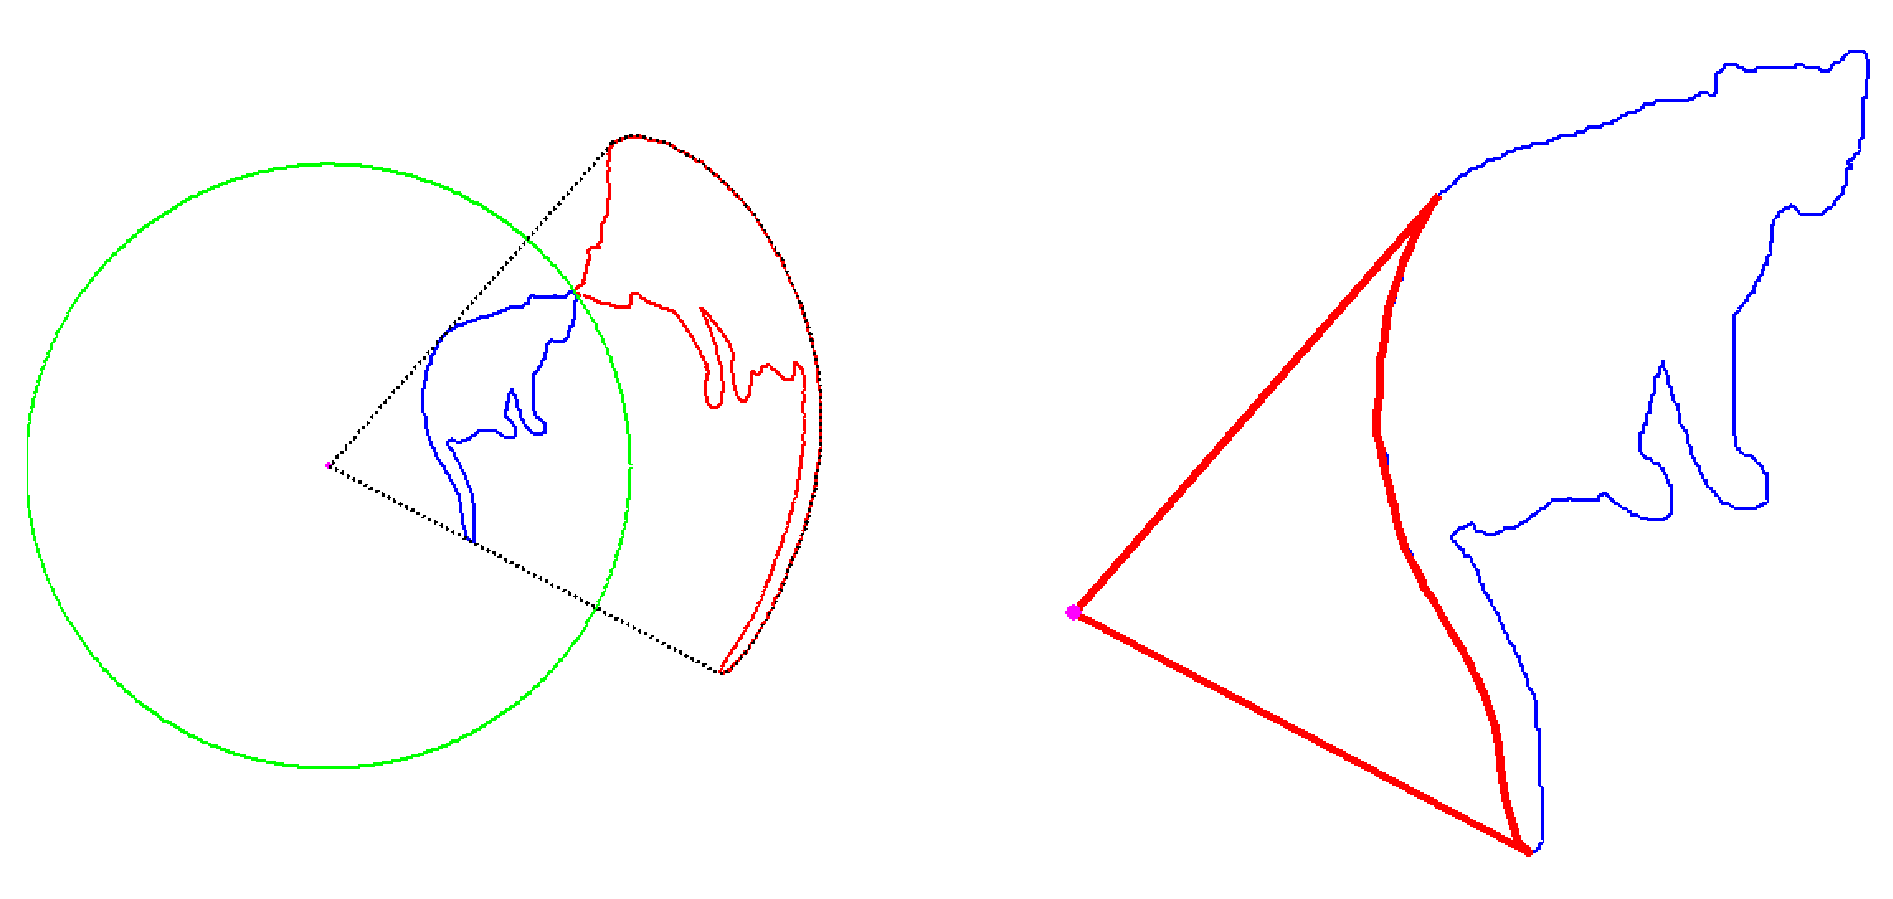
\includegraphics[scale=0.2]{img/hpr.png}
  \caption{HPR operator: on the left a spherical flipping (in red) of a curve (in blue) using a sphere (in green), on the right: a back projection of the convex hull.}
  \label{fig:hpr}
\end{figure}
\begin{figure}
  \centering
  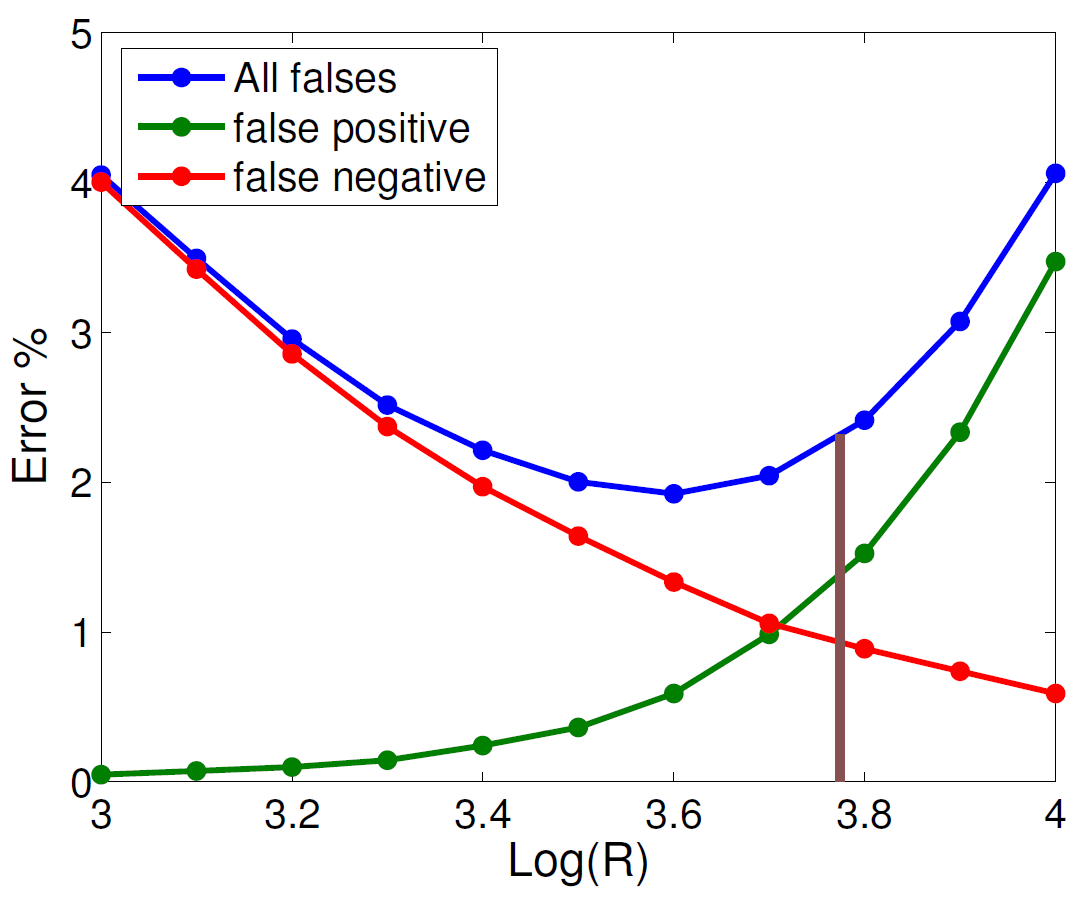
\includegraphics[scale=0.35]{img/hpr-r.png}
  \caption{The variation of: spherical inversion ray $R$, percentage of visibility detection error.}
  \label{fig:hpr-r}
\end{figure}

\begin{figure*}[t!]
  \centering
    \begin{subfigure}[t]{0.5\textwidth}
      \centering
	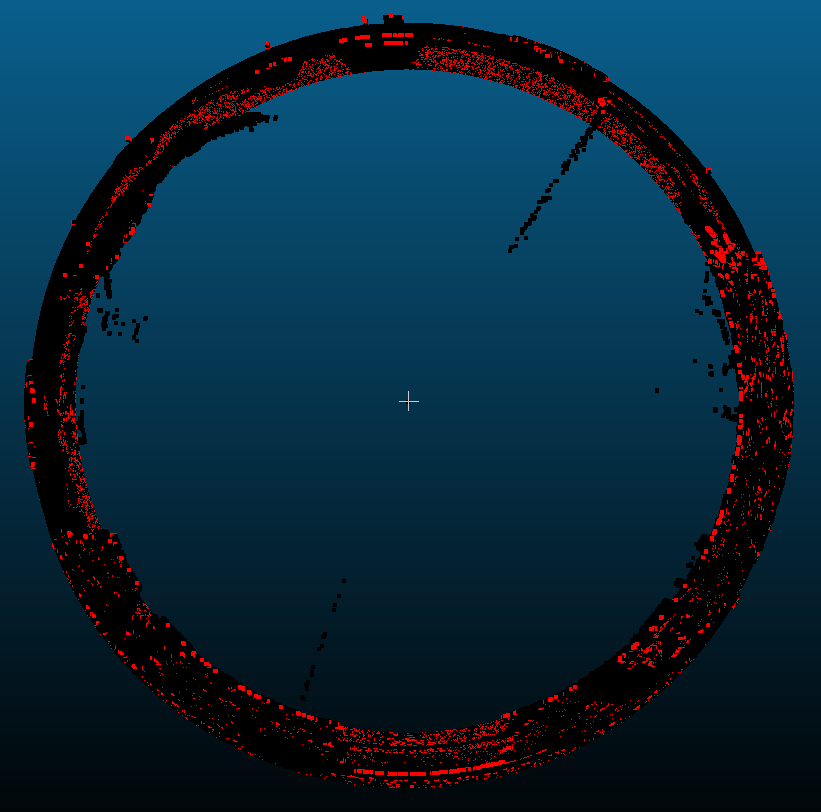
\includegraphics[height=3in]{img/hpr1.png}
    \end{subfigure}%
    ~
    \begin{subfigure}[t]{0.5\textwidth}
      \centering
	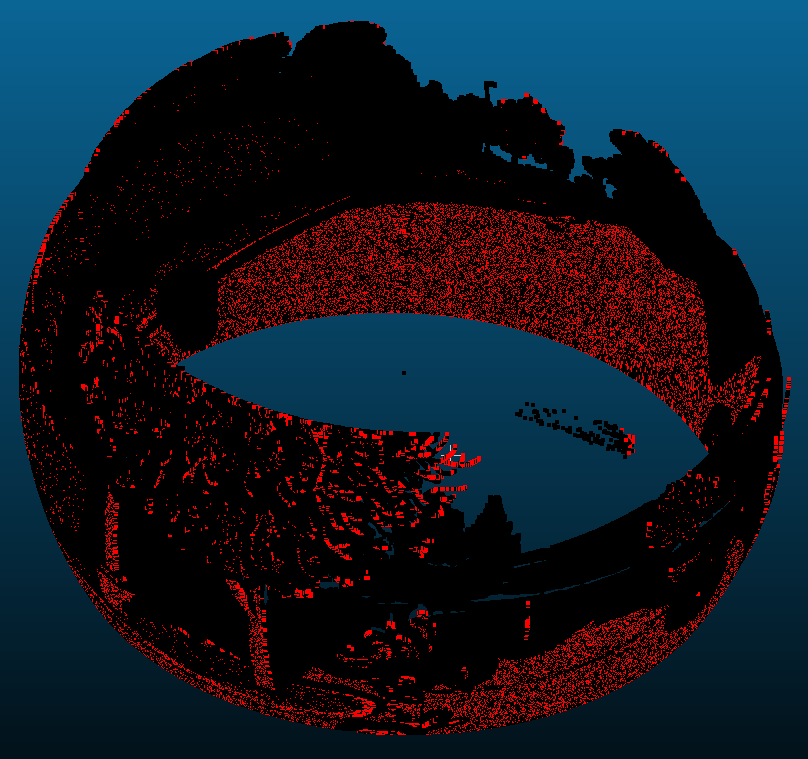
\includegraphics[height=3in]{img/hpr2.png}
    \end{subfigure}
    \caption{Different point of views of the spherical inversion of the Figure~\ref{fig:highdens} using $R = R_\text{max}$.}
    \label{fig:hpr1}
\end{figure*}
\begin{figure}
  \centering
  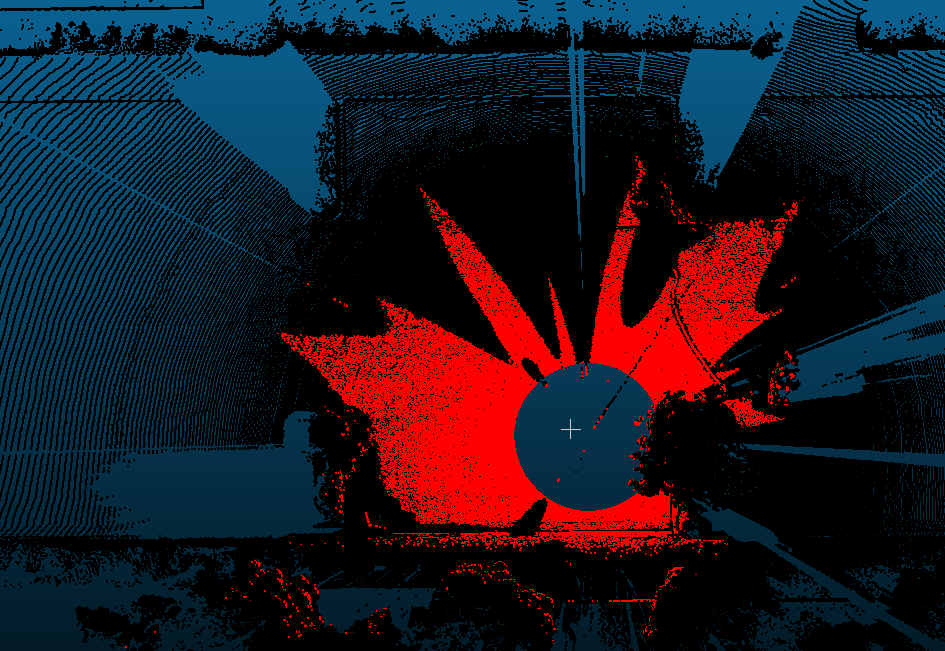
\includegraphics[scale=0.6]{img/hpr4.png}
  \caption{A topview of the visibile points after back propagation of convex hull computation (Figure~\ref{fig:hpr1}).}
  \label{fig:hpr4}
\end{figure}
\begin{figure}
  \centering
  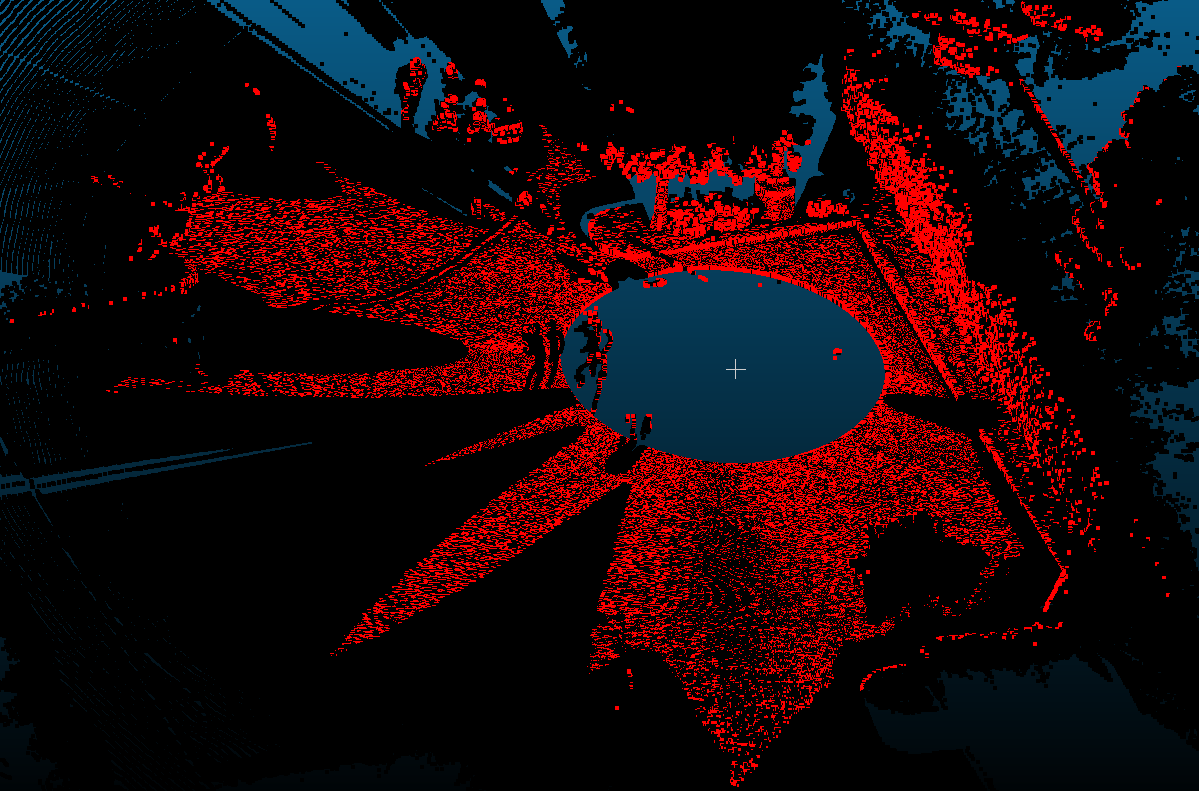
\includegraphics[scale=0.45]{img/hpr3.png}
  \caption{Another view of the visibile points after back projection of convex hull computation (Figure~\ref{fig:hpr1}).}
  \label{fig:hpr3}
\end{figure}


Figure~\ref{fig:hpr} shows both operation results\footnote{This result comes from the paper}. On the left is performed a spherical flipping (the inversion) of the point cloud, centered at the viewpoint $C$. In this example, the ray $R$ of the sphere seems to be $R_\text{max}$: \emph{the distance from $C$ to the furthest point}. However, the HPR authors suggest to use a second viewpoint (the opposite of the current viewpoint, its reflection about center of mass of the point cloud) and vary $R$ while maximizing the number of points considered visible by a unique viewpoint. Figure~\ref{fig:hpr-r} shows on the same plot, for a particular point cloud, the estimated $R=R_\text{opt}$ (in brown) and the percentage or error of the method while varying $R$.

Figures \ref{fig:hpr1}, \ref{fig:hpr3} and \ref{fig:hpr4} give an idea of how the HPR method behaves with LiDAR point clouds. As you can see in Figure~\ref{fig:hpr3} and Figure~\ref{fig:hpr4}, it is able to detect visible points within a small distance to the scanner location but quicly has difficulties when going away.

Although this method is simple, has only meaningful computations and an interesting complexity $\mathcal{O}(n\log{}n)$, it is not robust enough against noisy point clouds, in particular LiDAR ones. With a small $R$, visible points may be marked as non-visible by HPR. On the contrary, with a large $R$, non-visible points may be considered as visible. Moreover, this method handles poorly concave forms; it requirs a low curvature in case of concavity.


\subsection{\emph{Visibility of Noisy Point Cloud Data}}
\label{subsc:noisy}
As previously said, the \emph{Visibility of Noisy Point Cloud Data}~\cite{vis2} paper describes some improvements of \emph{Direct visibility of point sets}~\cite{vis1} for a better handling of noise and concave surfaces in point clouds.

\subsubsection{Overview}
\begin{figure}
  \centering
  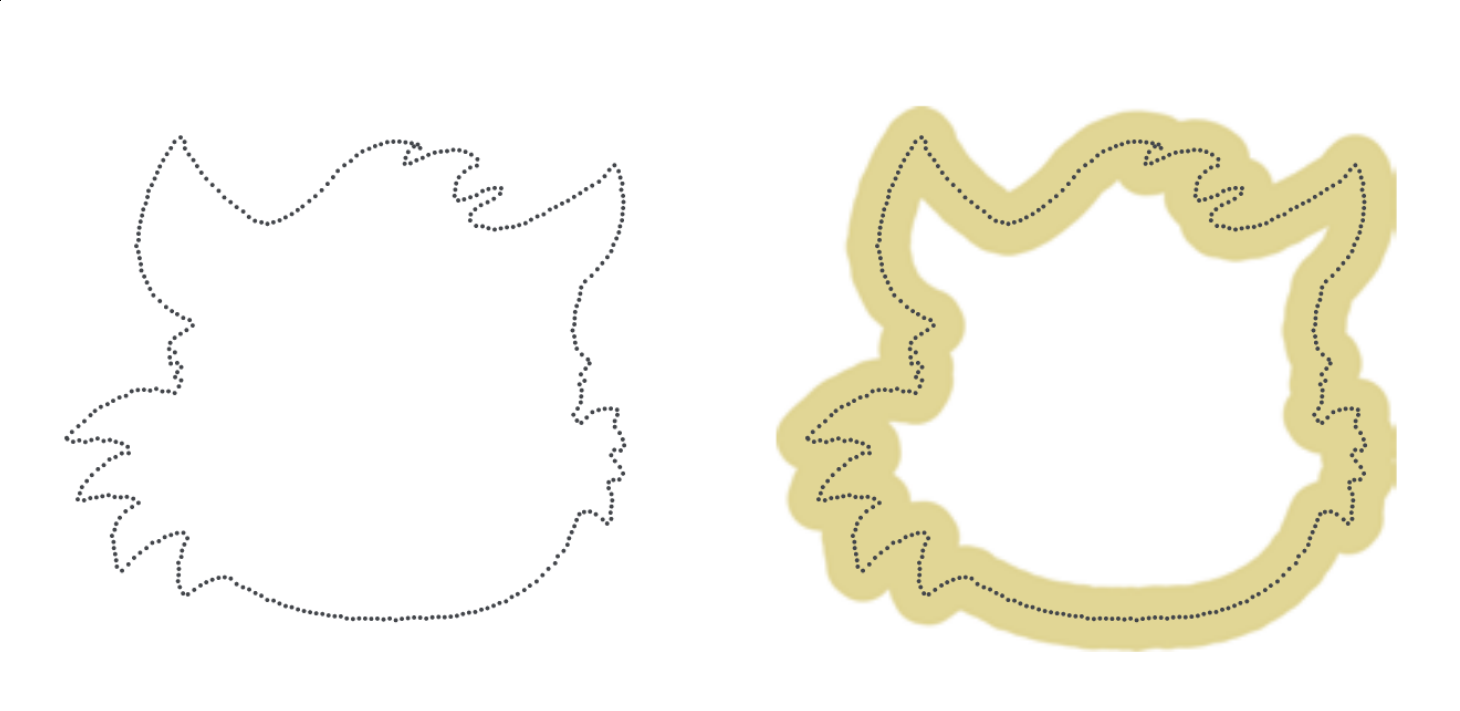
\includegraphics[scale=0.2]{img/epsilon.png}
  \caption{Region space (in yellow) from which the visibility cannot be reliably estimated, this is a guard zone.}
  \label{fig:epsilon}
\end{figure}

Noise in point clouds can be observed through perturbations of the convex hull. A noise is a movement of a point toward a direction. A noisy point cloud can be expressed as:
\begin{equation*}
  P^\sigma = \left\lbrace p_i + \sigma n_i | p_i \in P  \right\rbrace
\end{equation*}
where $n_i$ is a unit vector oriented in a uniformy chosen random direction and $\sigma$ a uniform random variable over the rand $[0, a]$. The \cite{vis2} paper explains some experiences and mathematical proof leading to:
\begin{itemize}
  \item a guard band on the convex hull which helps to consider as visible all points closer than $2 \times \epsilon_{\text{max}}$ to the convex hull. The value of $\epsilon_\text{max}$ is the maximum noise of $P^\sigma$ in the inverted domain.
    \begin{equation*}
      \epsilon_\text{max} = \left( \frac{4R}{a_\text{min} - \sigma} - 1 \right) \sigma
    \end{equation*}
    where $a_\text{min}$ is the distance from $C$ and the closest point in $P$.
  \item a boundary on the $R$ value that must be respected:
    \begin{equation*}
      ma_{\text{max}} \leq R \leq \left( \frac{\alpha D}{2 \sigma} + 1 \right) \left( \frac{a_{\text{min}} - \sigma}{4} \right)
    \end{equation*}
    where $D = a_\text{max} - a_\text{min}$ is the diameter of the point cloud and $m$ a value describing the surface form. When $m = 1$ the local region is convex, if $m > 1$ it is concav.
  \item A guard zone around the noisy point cloud that rejects viewpoints closer than the treshold. This threshold can be observed in Figure~\ref{fig:epsilon}. It depends on the point cloud, this is just a particular case.
    \begin{equation*}
      a_\text{min} \geq \frac{\left(4m + \frac{\alpha}{2} \right) D + \alpha}{\left(\frac{\alpha D}{2 \sigma} - (4m - 1)\right)}
    \end{equation*}
  \item an iterative method for concavity robustness. It varies $R$ value within the range. For each $R$ value it computes points visibility and update points weight based on the number of times they are tagged as visible. The idea is that high curvatures becore visible at higher values while others (convex, oblique, planar) are consistently visible. Thi is the function $f$ used in the Algorithm~\ref{alg:RobustHPR}.
\end{itemize}

The algorithm is shown in Algorithm~\ref{alg:RobustHPR}. Note that the function $f$ (which computes the ray $R$) is not formally written. It is the last bullet point above on the improvements of \cite{vis2} over \cite{vis1}. Instead it is describe above. Of course, the following algorithm is called for each scanner location $C$. When a point is seen by multiple scanners, we choose the closer one.

\begin{algorithm}[tb]
  \SetAlgoVlined
  \DontPrintSemicolon
  \SetKw{Report}{report}
  \SetArgSty{}
  \SetKwFunction{RobustHPR}{RobustHPR}
  \SetKwProg{Fn}{Function}{:}{}
  \Fn{\RobustHPR{$P$, $C$}}{
    \KwIn{
      \begin{itemize}
        \item a set of points $P = \left\lbrace p_i \mid i \in [0, s]  \right\rbrace$,
        \item the viewpoint $C$.
      \end{itemize}
    }
    \KwOut{a the set $V$ of visible points}
    \;
    $P' \gets \emptyset$ \tcp{contains inverted points}
    $\Delta' \gets \emptyset$ \tcp{contains inverted hidden points}
    $R \gets f(P, C)$\tcp{Compute the spherical inversion ray $R$}
    \;
    \tcp{spherical inversion}
    \ForEach{$p_i \in P$}{
      $p_i' \gets p_i + 2 \left( R - \left\lVert p_i  \right\rVert  \right) \frac{p_i}{\left\lVert p_i \right\rVert}$\;
      $P' \gets P' \cup \left\lbrace p_i' \right\rbrace$
    }
    \;
    \tcp{compute the convex hull of $P' \cup \left\lbrace C \right\rbrace$ in order to put aside visible points}
    $\Delta' \gets \text{convex\_hull}(P' \cup \left\lbrace C \right\rbrace)$\;
    \;
    \tcp{Catch all points within a $2 \times \epsilon_\text{max}$ distance form the convex hull points}
    $\epsilon_\text{max} \gets \left( \frac{4R}{a_\text{min} - \sigma} - 1 \right) \sigma$\;
    \ForEach{$p_i' \in \Delta'$}{
      \ForEach{$p_j' \in \Delta'$ belonging to the $50$ nearest points of $p_i'$}{
        \If{$\left\lVert p_i' - p_j' \right\rVert \leq 2\epsilon_\text{max}$}{
          $\Delta' \gets \Delta' \cup \left\lbrace p_j' \right\rbrace$\;
        }
      }
    }
    \;
    \tcp{Back projection of hidden points}
    $\Delta \gets \left\lbrace p_i \in P \mid p_i' \in \Delta' \right\rbrace$\;
    \;
    \Return{$ P \setminus \Delta $}\;
  }
  \caption{The robust HPR algorithm.\label{alg:RobustHPR}}
\end{algorithm}

\subsubsection{Results and discussions}
\begin{figure}
  \centering
  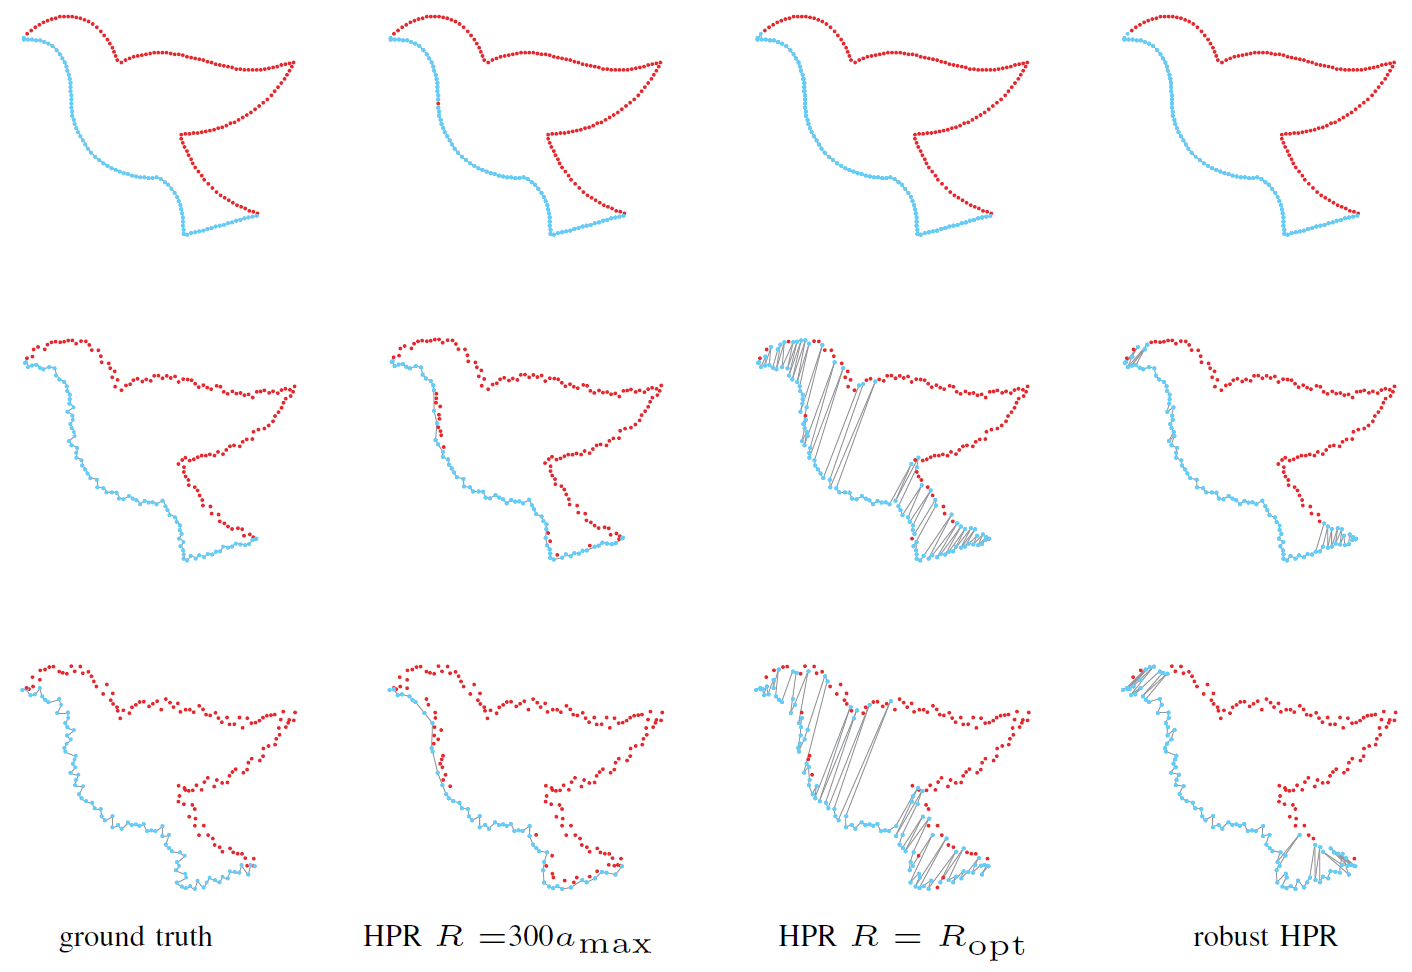
\includegraphics[scale=0.35]{img/rhpr-result.png}
  \caption{Result comparing HP$R_\text{max}$, HP$R_\text{opt}$ and Robust HPR.}
  \label{fig:rhpr-result}
\end{figure}

Figure~\ref{fig:rhpr-result} shows some results comparing this method (Robust HPR) with the original methods, one using $R = R_\text{max}$ and the other $R = R_\text{opt}$. It may be observed that Robust HPR achieves better results than the others. In our case, this has also been observed. However, it is still not robust enough against LiDAR point cloud noises. This is what leads us toward a custom approach described in Section~\ref{sc:custom}.

FIXME: Add pictures of the algorithm on Monday!!!

\section{A custom disk-based approach}
\label{sc:custom}
This section describes our custom \emph{disk-based} approach to resolve visibility in point clouds.

\subsection{Overview}
\label{subsc:custom-overview}
This method reduces the point cloud visibility problem to ray casting and intersection computations. It assigns to each point $p_i$ a \emph{disk}. A \emph{disk} is defined as a tuple $\left\langle p_i, r_d, \vec{n} \right\rangle$. It is computed as follows for a specific point $p_i$:
\begin{itemize}
  \item $p_i$ becomes the center of the disk,
  \item $r_d$ is the mediane distance to the $50$ nearest points of $p_i$,
  \item $\vec{n}$ is the normal at $p_i$ computed via a PCA (Section~\ref{subsc:pca}) applied on the $50$ nearest points of $p_i$, including itself.
\end{itemize}

Our custom approach can be compared to ray tracing as it casts a ray between all possible combination pairs of point $p_i$ and viewpoint $c_k$. We use the CGAL library~\cite{cgal} for collision detection. We define our custom Eigen \emph{Disk} type and specify how to detect intersections between a ray and a disk. Basically, a ray $r_a$ intersects a disk $d_j$ when the distance between its projection on the underlying disk plane and the disk center is lower than the
disk's ray $r_d$. Each time a ray is casted, a tuple $\left\langle v, n, d, k \right\rangle$ is saved. It contains:
\begin{itemize}
  \item a boolean $v$ telling if $p_i$ is visible from $c_k$,
  \item the number $n$ of collisions of $r_a$,
  \item the distance $d$ from $p_i$ and $c_k$,
  \item the scanner identifier $k$.
\end{itemize}

For each point, we cast all possible combination of rays with the viewpoints $c_k$. This gives multiple tuples. These tuples are sorted following this rule:

Consider two tuples $\left\langle v_1, n_1, d_1, k_1 \right\rangle$ and $\left \langle v_2, n_2, d_2, k_3 \right\rangle$ being compared. If one and only one tuple has a positive $v$, it is positionned before the other tuple. Otherwise we compare $n_1$ and $n_2$. If $ | n_1 - n_2 | > 2 $, the tuple having less collision is positionned before. Otherwise, we use a third criteria: the distance from the scanner which puts before, tuples with closer scanners. if a tuple has at least two collisions less than the other, it comes before. The sorting criteria have been found empirically. After sorting them out, the tuple at the position $0$ contains the scanner identifier associated to $p_i$.

\subsection{Implementation}
Algorithm~\ref{alg:disk-based} shows our custom algorithm for computing visibility in point clouds, especially LiDAR ones. As explained in Section~\ref{subsc:custom-overview}, we iterate over all points, all scanners, casts a ray between each pair combination possible and detects collisons. Actually, we use an improved version of this algorithm which assign multiple disks with different rays to each point. The idea is to have more different tuple candidates before sorting them. Clearly, this
slows the algorithm in a significant way, but instead, helps to have better visibility results.
\begin{algorithm}[tb]
  \SetAlgoVlined
  \DontPrintSemicolon
  \SetKw{Report}{report}
  \SetArgSty{}
  \SetKwFunction{DiskBasedVis}{DiskBasedVis}
  \SetKwProg{Fn}{Function}{:}{}
  \Fn{\DiskBasedVis{$P$, $C$}}{
    \KwIn{
      \begin{itemize}
        \item a set of points $P = \left\lbrace p_i \mid i \in [0, s]  \right\rbrace$,
        \item a set of viewpoints $C = \left\lbrace c_k \mid k \in [0, s_c] \right\rbrace$.
      \end{itemize}
    }
    \KwOut{a visibility Map $\langle i, j\rangle$ where $i$ and $j$ are respectively point and scanner unique identifiers.}
    \;
    $R \gets \emptyset$\;
    \ForEach{$p_i \in P$}{
      $V_\text{info} \gets \emptyset$ \tcc{Vector of $\left\langle v, n, d, k \right\rangle$ where $n$ is the number of intersection, $d$ the distance between $p_i$ and $c_k$, and finally $j$ the viewpoint identifier.}
      $\Delta \gets \emptyset$ \tcc{Vector of disk collisions $\left\langle p_j, \vec{n}_j \right\rangle$ where $p_j$ is the collided point$-$ center of its associated disk and $\vec{n}_j$ the disk's normal}
      \;
      \ForEach{$c_k \in C$}{
        $r_\text{ray} \gets p_i - c_k$ \tcp{the ray/vector from $c_k$ to $p_i$}
        $d_\text{ik} \gets \left\lVert r_\text{ray} \right\rVert$ \tcp{distance between the point $p_i$ and the viewpoint $c_k$}
        $v \gets \top$ \tcp{set to $\top$ as $p_i$ is considered visible at the beginning}
        $\Delta \gets$ intersected\_disks$(r, P, C)$\;
        \;
        \ForEach{$\left\lbrace p_j, \vec{n}_j  \right\rbrace \in \Delta $}{
          $d_\text{ij} \gets \left\lVert p_j - p_i  \right\rVert$ \tcp{distance between the point $p_i$ and the collided point $p_j$}
          $d_\text{kj} \gets \left\lVert c_k  - p_j  \right\rVert$ \tcp{distance between the collided point $p_j$ and the viewpoint $c_k$}

          \If{$v \land d_\text{ij} < d_\text{ik} \land\ \neg( d_\text{kj} \leq 0.1\ \land | \vec{n}_j \times \vec{n}_i| > 0.6 )$}{
            $v \gets \bot$\;
            \Break
          }
        }
        $ V_\text{info} \gets V_\text{info} \cup \left\lbrace \left\langle v, \text{size\_of}(\Delta), d_\text{ik}, j \right\rangle \right\rbrace $\;
      }
      \;
      $V_\text{info} \gets \text{sort}(V_\text{info})$ \tcp{sort $V_\text{info}$ based on $v$, $\text{size\_of}(\Delta)$ and $d_\text{ik}$}
      $v \gets \text{first element of} V_\text{info}$\;
      $R \gets R \cup \left\lbrace \left\langle i, v_j \right\rangle \right\rbrace $\;
    }

    \;
    \Return{$R$}\;
  }
  \caption{A custom disk-based approach for visibility in point clouds.\label{alg:disk-based}}
\end{algorithm}


\subsection{Results and discussions}
\begin{figure}
  \centering
  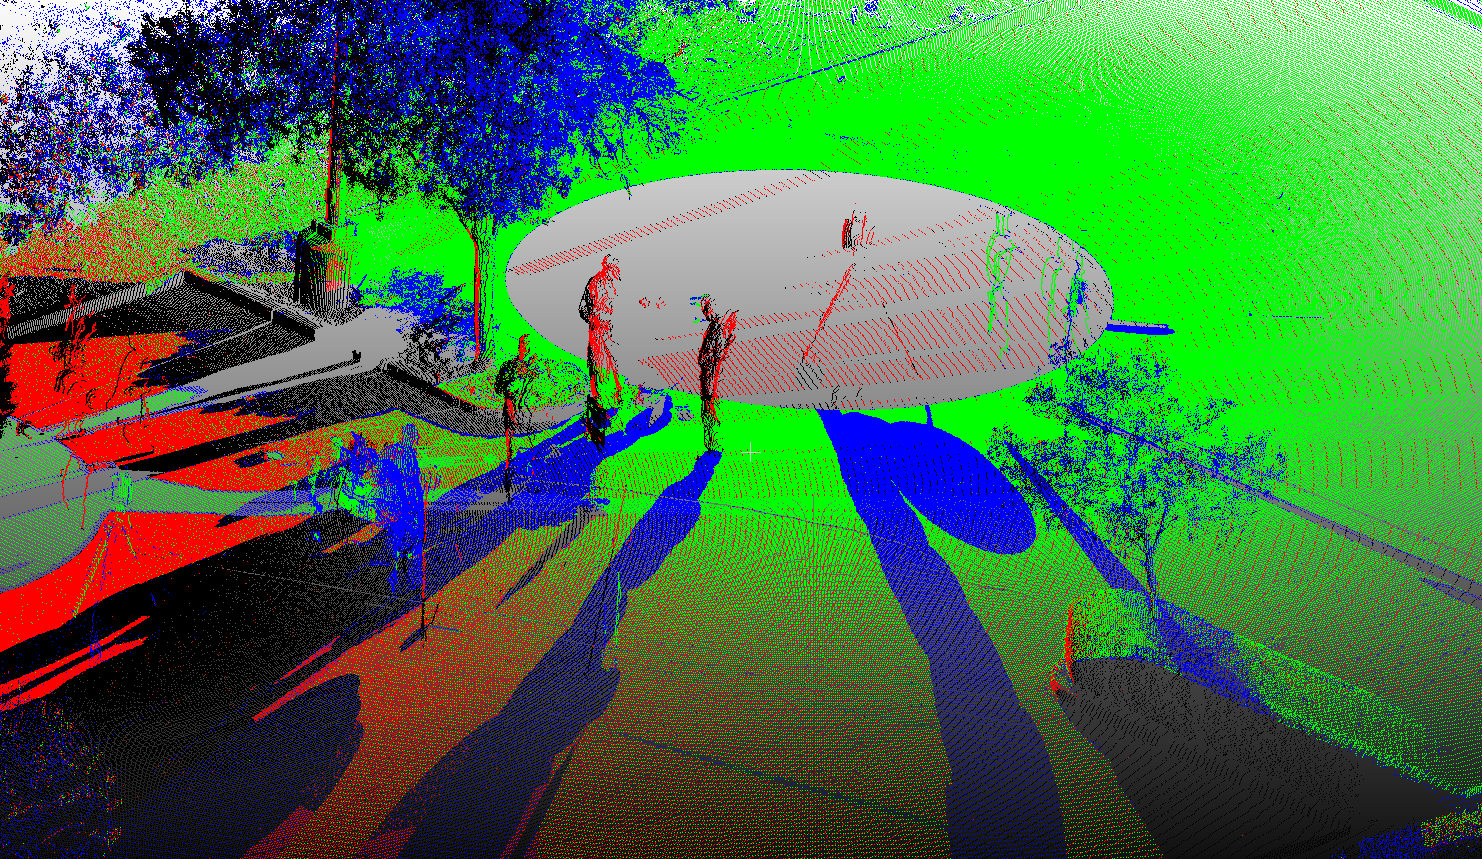
\includegraphics[scale=0.3]{img/positive-negative.png}
  \caption{A visual representation of the Parking point cloud (scanner 0), sowing Table~\ref{fig:positive-negative} data. Find true positive in green, true negative in black, false positive in red and false negative in blue}
  \label{fig:positive-negative}
\end{figure}
\begin{figure}
  \centering
  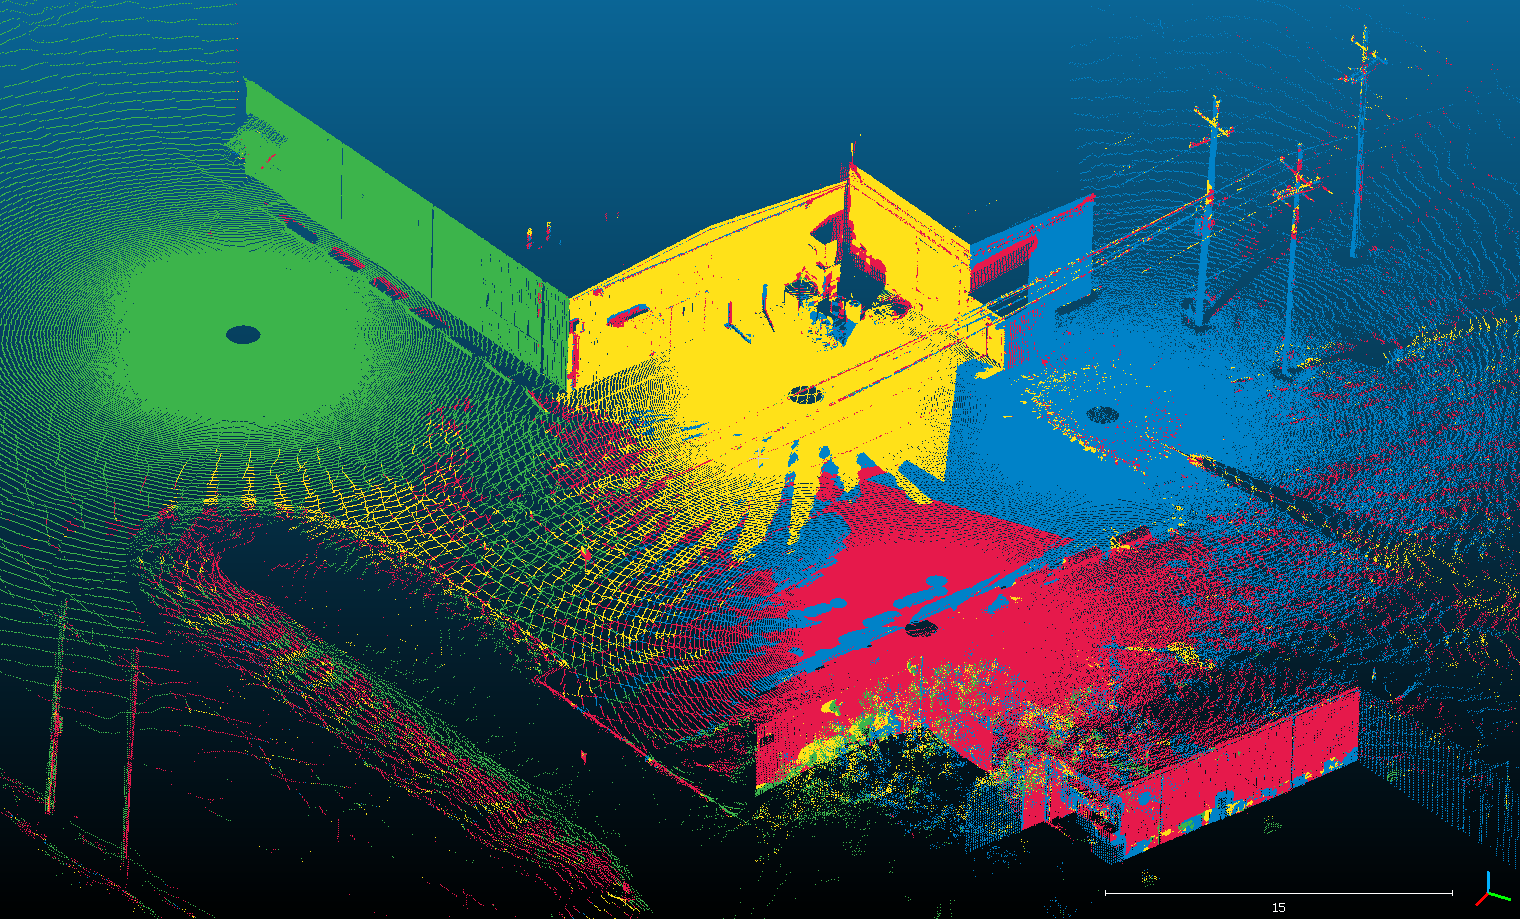
\includegraphics[scale=0.35]{img/custom-result1.png}
  \caption{A first \emph{DiskBasedVisibility} result: points colored with the same color are assigned to the same viewpoint--scanner location. There are four (4) colors, thus four (4) scanners in the point cloud.}
  \label{fig:custom-result1}
\end{figure}
\begin{figure}
  \centering
  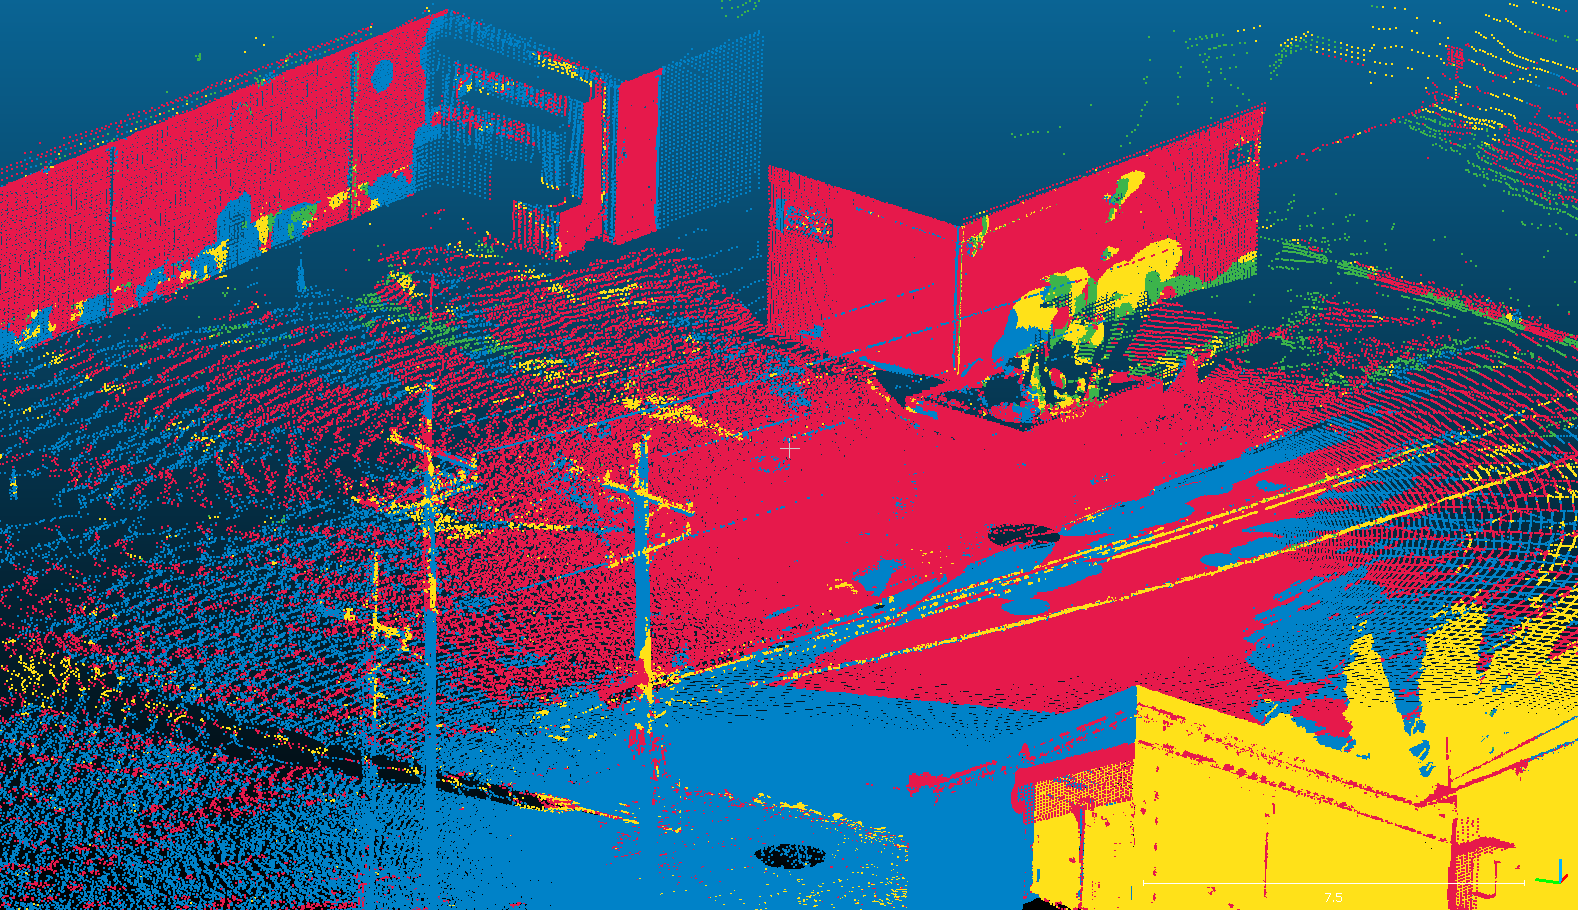
\includegraphics[scale=0.35]{img/custom-result2.png}
  \caption{Another view of Figure~\ref{fig:custom-result1} result: points colored with the same color are assigned to the same viewpoint--scanner location. There are four (4) colors, thus four (4) scanners in the point cloud.}
  \label{fig:custom-result2}
\end{figure}
\begin{figure}
  \centering
  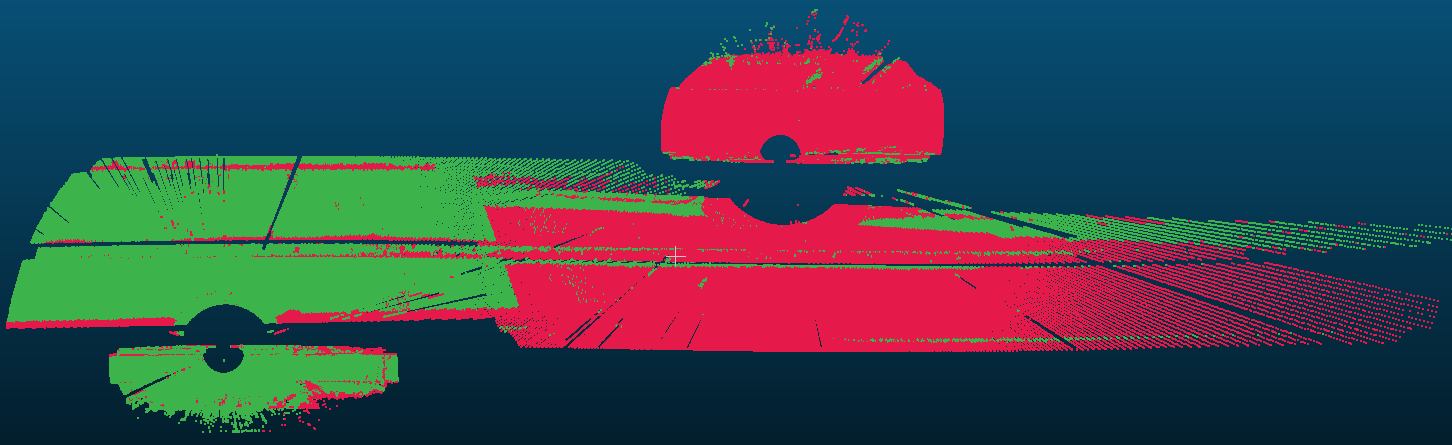
\includegraphics[scale=0.35]{img/custom-result3.png}
  \caption{A second \emph{DiskBasedVisibility} result: points colored with the same color are assigned to the same viewpoint--scanner location. There are two (2) colors, thus two (2) scanners in the point cloud.}
  \label{fig:custom-result3}
\end{figure}
\begin{figure}
  \centering
  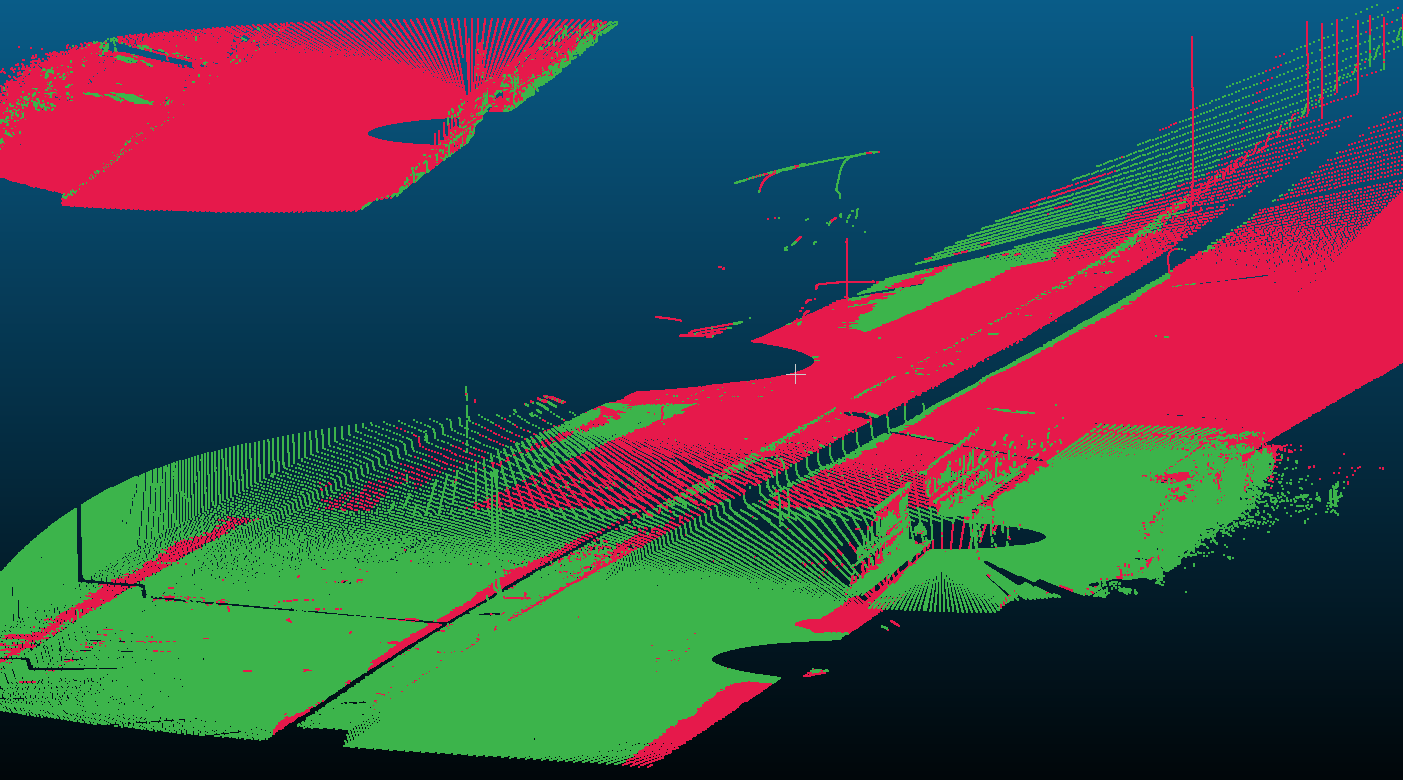
\includegraphics[scale=0.35]{img/custom-result4.png}
  \caption{Another view of the custom visibility algorithm result on the same point cloud $P_2$: points colored with the same color are assigned to the same viewpoint--scanner location. There are two (2) colors, thus two (2) scanners in the point cloud.}
  \caption{Another view of Figure~\ref{fig:custom-result3} result: points colored with the same color are assigned to the same viewpoint--scanner location. There are two (2) colors, thus two (2) scanners in the point cloud.}
  \label{fig:custom-result4}
\end{figure}
\begin{figure}
  \centering
  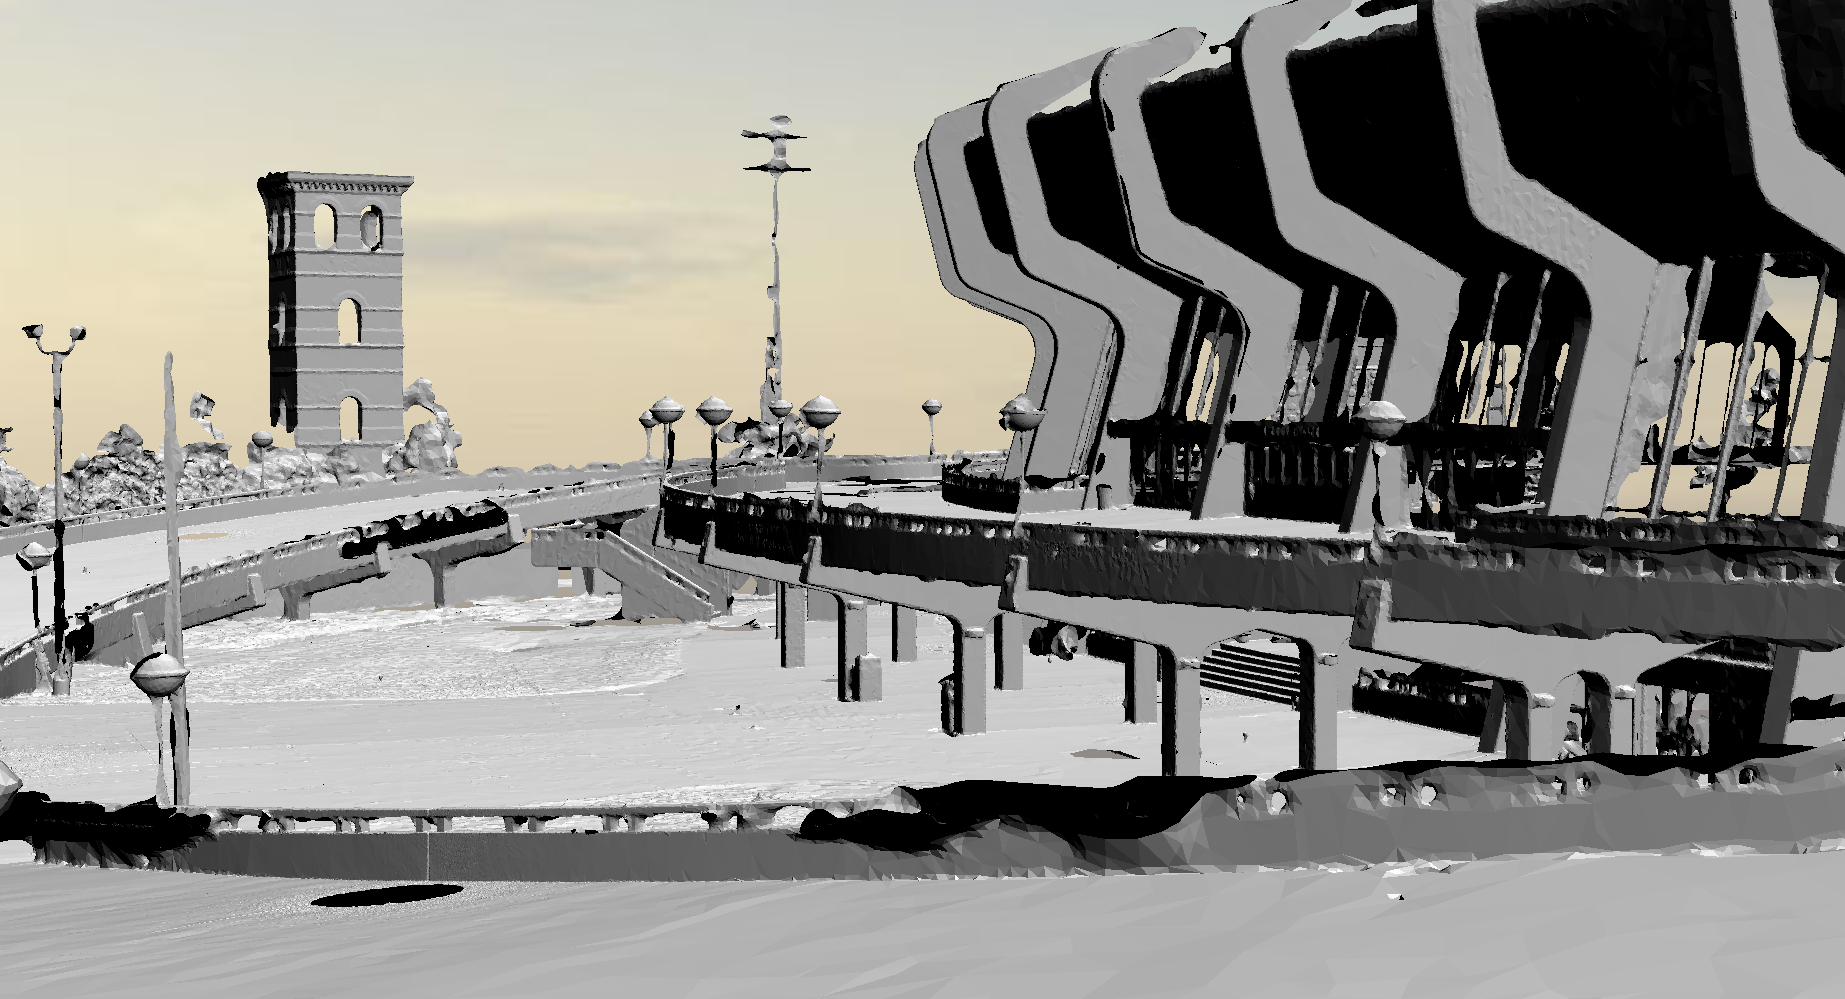
\includegraphics[scale=0.35]{img/complete-result1.png}
  \caption{A 3D reconstruction view of a point cloud after using \emph{ScanFinder} and \emph{DiskBasedVisivility}.}
  \label{fig:complete-result1}
\end{figure}
\begin{figure}
  \centering
  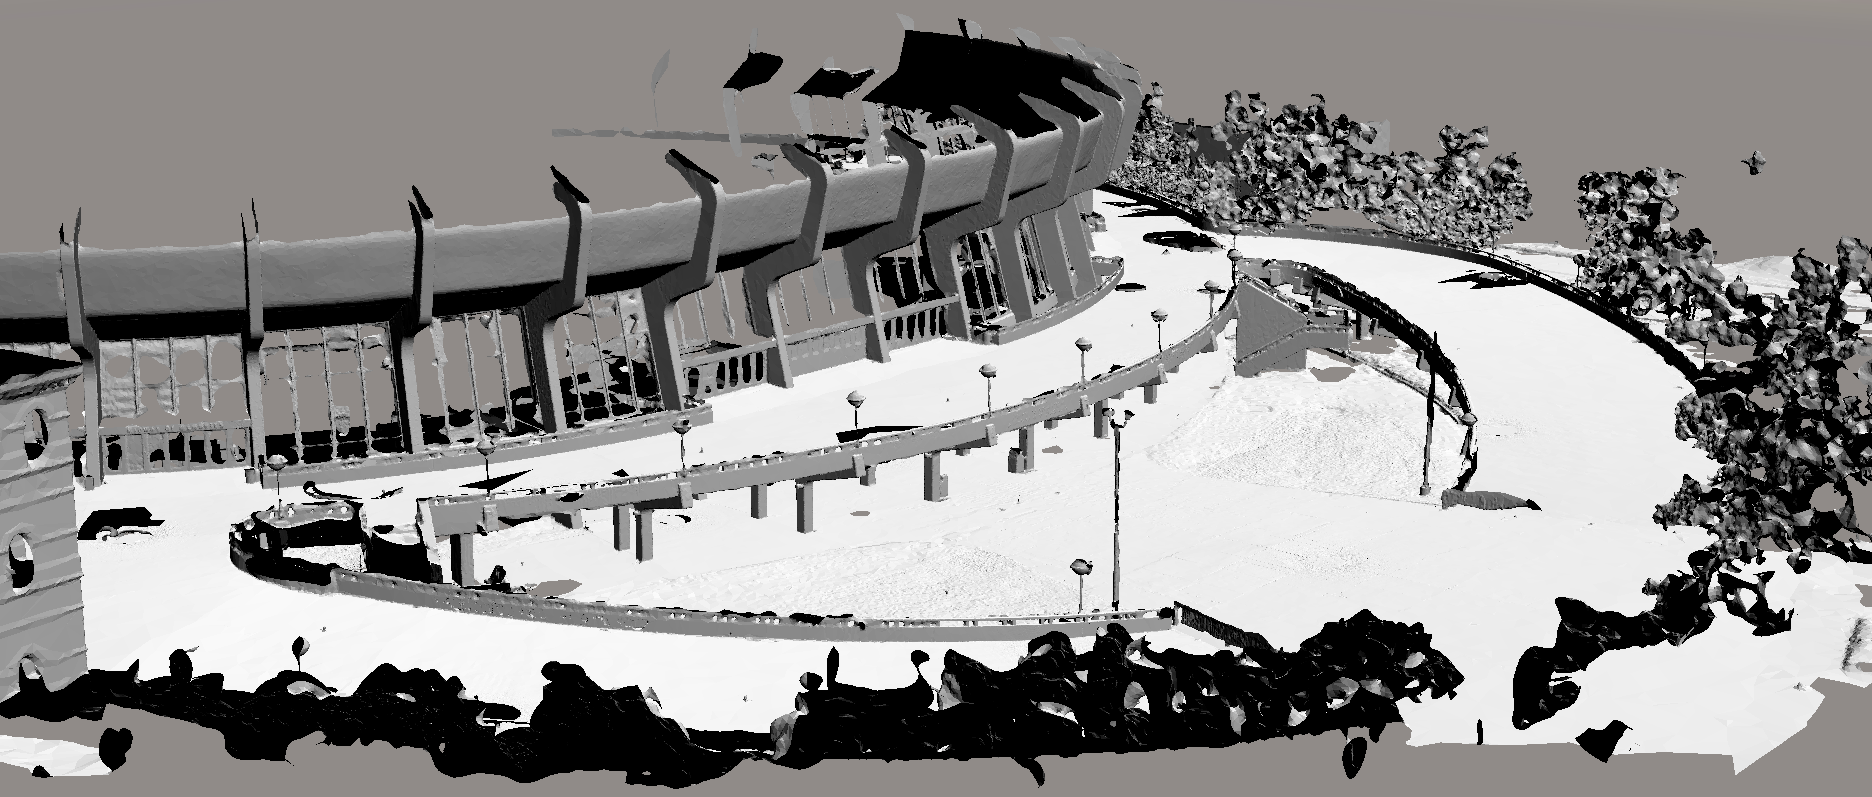
\includegraphics[scale=0.35]{img/complete-result2.png}
    \caption{Another 3D reconstruction view of the same point cloud as Figure~\ref{fig:complete-result1} after using \emph{ScanFinder} and \emph{DiskBasedVisivility}.}
  \label{fig:complete-result2}
\end{figure}

\begin{table}[]
  \centering
\begin{tabular}{l|c|c|c|c|c}
Point cloud                                 & Scanner & True Positive & False Positive & False Negative & True Negative \\\hline
Pump (604,638 points)                       & 0       & 604,638       & 0              & 0              & 0             \\\hline
\multirow{2}{*}{Parking (5,188,752 points)} & 0       & 2,135,577     & 372,473        & 413,596        & 2,267,106     \\
                                            & 1       & 2,267,106     & 413,596        & 372,473        & 2,135,577     \\\hline
\multirow{3}{*}{Road (2,220,166 points)}    & 0       & 693,574       & 34,946         & 34,109         & 1,457,537     \\
                                            & 1       & 60,050        & 695,844        & 685,682        & 778,590       \\
                                            & 2       & 55,119        & 680,633        & 691,632        & 792,782       \\\hline
\multirow{2}{*}{Ashlan (23,484,370 points)} & 0       & 558,423       & 11,486,621     & 11,047,445     & 391,881       \\
                                            & 1       & 391,881       & 11,047,445     & 11,486,621     & 558,423
\end{tabular}
  \caption{Some statistics on the visibility attribution on different point clouds. For each scan $c$ of each point cloud, we counted false negative (considered not visible by $c$ while they actually are), true negative (considered not visible and it is not), true positive (considered visible and it is) and false positive (considered visible while they are not).}
  \label{table:counts}
\end{table}

\begin{table}[]
  \centering
  \begin{tabular}{l|c|c}
    Point Cloud & Number of points & Error (percent) \\\hline
    Pump: & 604,638 &  0.19631 \\\hline
    Parking: & 5,188,752 & 2.70431 \\\hline
    Road: & 2,220,166 & 1.75293 \\\hline
    Ashlan8+11 & 23,484,370 & 0.69309
  \end{tabular}
  \caption{The percentage of error of our Disk-based approach on different point cloud sets with their respective sizes.}
  \label{table:vis-error}
\end{table}
Figure~\ref{fig:custom-result1} and Figure~\ref{fig:custom-result2} are two different views of our method results on a point cloud. In general the method seems to work well. Points near one scanner are coloured with a unique color. Figure~\ref{fig:custom-result2} shows a particular case where the method works well. Assume the current viewpoint as being at the scanner associated to the red color. The algorithm is able to detect that a wall far away (in blue) is hidden by a closer wall (in red). Figure~\ref{fig:custom-result3} and Figure~\ref{fig:custom-result4} shows two other views of another point cloud visibility result.

Table~\ref{table:counts} shows some statistics of our method for different point clouds. The first point cloud contains only one scanner. This is a particular case where we automatically attribute all points to it. Figure~\ref{fig:positive-negative} shows a view where each point is colored base on its category in Table~\ref{table:counts}. Although these measures are interesting, they ignore one important point. A point does not need to be assigned to its original scanner,
it only needs a scanner that sees it well. Some points in false positive and false negative may not be false, as long as the scanners to which they are attributed find the right normal orientations. We present in Table~\ref{table:vis-error} a more accurate measure. It computes the point cloud visibility, orient the normals and compare this orientation with the known correct one. Our method achieves good results. It has not more than $3$ percent error.

In summary, this custom approach meets all of our requirements instead of the running time. For instance, it almost took 6 days to compute visibility of a 2.5 GB point cloud with 135,069,108 points. This algorithm was written as a prototype in order to validate our intuitions, it has not been optimized yet. Several improvements can be made on the algorithm, such as tasks parallelization. The algorithm will certainly be optimized before being integrated to \CC.

To finish appropriately this Chapter and the previous one, you can find in Figure~\ref{fig:complete-result1} and Figure~\ref{fig:complete-result2} two views of a point cloud reconstructed using both \emph{ScanFinder} followed by \emph{DiskBasedVisibility}. Despite some errors, notably the trees reconstruction, the result goes beyond our expectations.
